\documentclass[conference]{IEEEtran}
\IEEEoverridecommandlockouts
\usepackage{cite}
% fontspec + the Persian font must come BEFORE newtxtext (which breaks fontspec lookups under XeTeX)
\usepackage{fontspec}
\newfontfamily\persianfont[Script=Arabic]{Noto Naskh Arabic}
\TeXXeTstate=1
% Persian examples, right-to-left, in a font that has the glyphs
\newcommand{\fa}[1]{{\persianfont\beginR #1\endR}}
\usepackage{amsmath}
\usepackage{newtxtext}
\usepackage{newtxmath}
\usepackage{algorithm}
\usepackage{algorithmic}
\usepackage{graphicx}
\usepackage{booktabs}
\usepackage{tikz}
\usepackage{xcolor}
\usepackage[hidelinks]{hyperref}
% numbers still to be filled from output/research/*.json are marked \RES{}
% Every red number is traceable to research/PROGRESS.md. For the submission version replace the next
% line by \newcommand{\RES}[1]{#1} (all numbers then print in black).
\newcommand{\RES}[1]{\textcolor{red}{#1}}
\renewcommand{\algorithmicrequire}{\textbf{Input:}}
\renewcommand{\algorithmicensure}{\textbf{Output:}}

\begin{document}

\title{Prompt Self-Extension: A Training-Free Fix for Short-Utterance Failures\\
in a CPU Persian Text-to-Speech Model}

\author{\IEEEauthorblockN{AUTHOR-1, AUTHOR-2}
\IEEEauthorblockA{AFFILIATION\\ EMAIL}}

\maketitle

\begin{abstract}
Small continuous-latent text-to-speech (TTS) models now run in real time on a CPU, but short inputs are their
weak spot. We study a 110M-parameter Persian model and make three points. (i)~\emph{Measurement:} the usual
judge, Whisper, hallucinates on short audio; on real two-second recordings it fails \RES{17\%} of correct
clips. Scoring with two recognisers and counting a failure only when both agree, the true short-unit failure
rate is \RES{4--10\%}, five to ten times lower than Whisper alone reports. (ii)~\emph{Post-processing:}
signal checks the engine gets for free (energy, duration, end-of-speech timing, latent self- and
cross-similarity, syllable counts) predict which \emph{units} are risky but cannot tell a failed take from a
good take of the same unit, so retries without a recogniser recover little. (iii)~\emph{Pre-processing:}
failures depend on how the voice prompt \emph{ends}. We propose \emph{prompt self-extension}: once per
voice, the model reads one neutral sentence in that voice, and every later take is conditioned on the
reference clip followed by that reading. Ending the prompt at the model's own completed sentence is the
mechanism: cutting the extension mid-sentence multiplies failures by \RES{3--10}, and placing the clip last
makes the model read the extension aloud. On held-out short sentences rendered through the full production
pipeline with three voices, self-extension halves failed renders (\RES{24 $\to$ 12} of \RES{900}; consensus
error \RES{3.2\% $\to$ 2.2\%}, 95\% CI of the difference \RES{[$-$1.7, $-$0.4]} points) and raises UTMOS for
every voice; on three new, tightly cut real clips it cuts failures from \RES{96} to \RES{19} of \RES{450},
and a clip cut mid-clause goes from \RES{44\%} to \RES{3\%} error. The method needs no training and adds no per-request cost; its small
speaker-similarity cost on some voices disappears when the extension take is chosen by speaker similarity.
With it, the engine's retries can be dropped, halving the generation work while remaining more accurate.
\end{abstract}

\begin{IEEEkeywords}
text-to-speech, Persian, robustness, voice prompt, inference-time methods, low-resource
\end{IEEEkeywords}

\section{Introduction}
Continuous audio language models (CALM) generate speech as a sequence of continuous codec latents
\cite{calm2025}; Pocket TTS distils such a model to a 100M-parameter student that runs faster than real
time on a laptop CPU \cite{pockettts2026}, and a community Persian student trained on 973\,h is available
\cite{farsiv2}. We use it, exported to ONNX, as the speech engine of a Persian--English assistant. Its
errors are not uniform: an assistant's short replies (\fa{«باشه»}, \fa{«ممنون از پیامتان»}) are exactly where it fails,
dropping final syllables or garbling the whole word.

Robustness of autoregressive TTS is usually bought with training: preference alignment and classifier-free
guidance \cite{koel2025}, fine-tuning on short phrases \cite{gepard2026}, or distilling ASR-verified
best-of-$N$ outputs back into the model \cite{asaria2026}. These need the training pipeline, data with
rights to use, and GPU time; for the released Persian student the 24-layer teacher it was distilled from is
not even public. We ask what can be done at inference time only, and answer two questions:

\begin{enumerate}
\item \textbf{Can post-processing catch failures without a recogniser?} We build a labelled corpus of
single takes and test every signal the engine sees for free. They identify risky units, not failed takes
(Sec.~\ref{sec:a}).
\item \textbf{Can the input be changed so the takes do not fail?} We show that how the voice prompt ends
drives short-unit failure and propose prompt self-extension, with an ordering rule that the model's
training explains (Sec.~\ref{sec:b}).
\end{enumerate}
Answering both required fixing the measurement first: we show that a single ASR judge overstates short-unit
failures several-fold and use a two-recogniser consensus instead (Sec.~\ref{sec:system}).

\section{Related work}
\textbf{Robust AR TTS.} Hallucinated, repeated and dropped content is a known failure of autoregressive
TTS \cite{koel2025,borodin2026repetition}. Asaria et al.\ remove most catastrophic failures with ASR
self-verification and distillation \cite{asaria2026}; GEPARD reports a systematic collapse on 1--2-word
inputs and fixes it by fine-tuning \cite{gepard2026}; LEMAS penalises repetition during decoding
\cite{lemas2026}; LoopGuard detects loops from token diversity in text LLMs \cite{loopguard2026}. All
detectors we know of either use a recogniser or discrete tokens; a continuous-latent model has neither.

\textbf{Context at inference time.} For long-form speech, MagpieTTS-LF steers attention across chunks
\cite{magpielf2026}, Liu et al.\ post-train boundary-aware streaming \cite{liu2026boundary}, and Lim et al.\
find that the acoustic prompt must stay in context while speaker similarity still decays
\cite{lim2026longer}. We study the prompt itself: its length and what it ends with.

\textbf{Persian TTS.} Open resources include ManaTTS \cite{manatts2025}, ParsVoice \cite{parsvoice2026},
homograph-aware G2P \cite{homorich2025} and the PARSA-Bench audio benchmark \cite{parsabench2026}.

\section{System and failure analysis}\label{sec:system}
\textbf{Model.} pocket-tts-farsi-v2 \cite{farsiv2} is a 6-layer CALM student (110M parameters) over 24\,kHz
Mimi latents at 12.5\,Hz. Text enters as Persian phonemes from a G2P model; English words are mapped to the
same phoneme set. Each unit is generated from a fresh state: \texttt{[BOS, voice prompt, text, latents\dots]}.
The voice prompt is a reference clip of at most 5\,s; in training it was the audio \emph{preceding} a random
word boundary of the same utterance, with the words after the boundary as text.

\textbf{Engine.} Text is split into sentences and phrases, then into units of at most 30 phoneme tokens by
dynamic programming over break costs (ezafe, verbs, \fa{«را»}). Each unit is generated up to three times; a
signal check (level, speech fraction, duration window, dead air) accepts a take or keeps the best of three.

\textbf{Corpus.} \RES{110} development sentences (short replies, casual, formal, numeric, mixed, English, long)
were planned exactly as in production, giving \RES{127} units; each was generated six times with each of three voices
(clips of 1.36\,s, 2.0\,s and 5.1\,s), without retries: \RES{2{,}286} takes. Each take is scored by
consonant-skeleton CER: consonants mapped to sound classes, vowels dropped on both sides, because Persian
script does not write short vowels.

\textbf{Two judges.} Whisper large-v3-turbo \cite{whisper2023} (beam 5, digits suppressed) is a poor judge of
short audio: on \RES{76} \emph{real} recordings of short Persian sentences (GPTInformal, CC0, mean
\RES{1.8}\,s) it charges skeleton CER \RES{0.188} and fails \RES{17\%} of them, often writing \fa{«موسیقی»}
(``music'') for speech. A character-level wav2vec2-CTC recogniser for Persian (no language model) fails
\RES{10.5\%} of the same clips (\RES{0.115}). On synthetic short takes the two judges correlate only
\RES{0.23}. We therefore report both and use a \emph{consensus} label: a take fails (CER $>0.3$) only if both
recognisers fail it, so a hallucination of either cannot fail a take. English units are judged by Whisper
alone.

\begin{figure}[t]
\centering
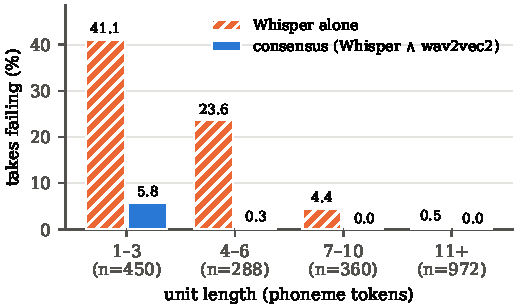
\includegraphics[width=\columnwidth]{figures/fig_judges.pdf}
\caption{Single-take failure rate (skeleton CER $>0.3$) by unit length on the development corpus
(\RES{2{,}070} Persian takes, three voices): Whisper alone vs.\ the two-recogniser consensus.}
\label{fig:judges}
\end{figure}

\textbf{Findings.} Under the consensus label \RES{1.3\%} of the \RES{2{,}070} Persian takes fail, all of
them in units of at most six phoneme tokens and nearly all in units of 1--3 tokens (\RES{5.8\%} of those
takes; none of the \RES{972} takes of more than ten tokens). Whisper alone would report \RES{12.3\%} overall
and \RES{41\%} for 1--3-token units (Fig.~\ref{fig:judges}). Most
failures are deletions (\RES{19} of \RES{27}), and the frames generated after end-of-speech are silent: the
model, not the trimming, drops the ending. Short-unit error depends on the voice prompt (\RES{0.060 / 0.027 /
0.016} for the 1.36 / 2.0 / 5.1\,s clips), and the two clips that ship with the engine end 0.02\,s and 0.07\,s
after their last phoneme.

\section{Post-processing without a recogniser}\label{sec:a}
A retry loop is only as good as its accept/reject test. We computed, for every take, the signals an engine
has for free.
\emph{Signal QC} (the engine's rule): level, fraction of frames with speech energy, speech duration against
a token-rate window, longest dead-air run.
\emph{Timing:} end-of-speech step per vowel of the target, speech seconds per vowel, the number of syllable
nuclei (peaks of the 0.3--2.5\,kHz envelope) against the number of vowels in the phonemes.
\emph{Latent recurrence:} the strongest off-diagonal stripe of the cosine self-similarity of the take's
latents over speech frames (0.64\,s window, lag $\ge$ 0.48\,s), which a take that says a stretch twice
produces; and the strongest stripe of its cross-similarity with the prompt's latents, which a take that
replays the prompt produces.
A logistic regression on these signals is trained on the development corpus and evaluated by
case-grouped cross-validation.

\textbf{Units, not takes.} With consensus labels the combined detector reaches a case-grouped
cross-validated AUC of \RES{0.88}, but its strongest input is the unit length itself (AUC \RES{0.94} alone).
Holding the unit fixed --- over all pairs of a failed and a good take of the same unit and voice --- the best
single signals reach \RES{0.66} (speech fraction) and \RES{0.67} (end-of-speech step per vowel), the engine's
rule \RES{0.58}, latent recurrence and prompt similarity \RES{0.48--0.57}. The signals know which units are
hard, not which take failed. They are not blind in general: on \RES{300} takes made with the clip placed
after the extension (Sec.~\ref{sec:b}), \RES{95\%} of which fail (the model reads the prompt's sentence), the prompt cross-similarity
separates them from normal takes of the same units with AUC \RES{0.98}. Natural failures of this engine are
different --- short deletions --- and those the signals do not see. The engine's rule is also badly calibrated: it rejects \RES{29\%} of takes,
\RES{96\%} of them good ones.

\textbf{Selection.} Table~\ref{tab:sel} replays retry policies on the six stored takes per unit. The
engine's rule spends \RES{49\%} more generation for \RES{2.35\%} $\to$ \RES{2.15\%} mean CER; keeping the
longest take (deletions dominate) or the latent DTW medoid does not help; an oracle choosing among the same
takes halves the error. The headroom exists, but finding it needs a recogniser. The held-out bench corpus (79 cases, four
takes per unit, \RES{1{,}632} Persian takes) repeats the picture: \RES{0.9\%} of takes fail, \RES{13} of
\RES{15} by deletion in units of $\le$6 tokens; the dev-trained detector falls to AUC \RES{0.78} and its
threshold does not transfer; retries move the error from \RES{2.89\%} to \RES{2.75\%} against an oracle's
\RES{1.23\%}. Since the failures sit in short units, we turn to the input.

\begin{table}[t]
\caption{Retry policies replayed on stored takes (dev, Persian, \RES{345} unit$\times$voice groups,
consensus CER / failure rate)}\label{tab:sel}
\centering
\begin{tabular}{lcc}
\toprule
policy & takes/unit & CER / fail \\
\midrule
first take & 1 & \RES{.0235 / 0.9\%} \\
engine signal QC (3 max) & \RES{1.49} & \RES{.0215 / 0.6\%} \\
ASR-free detector (3 max) & \RES{1.31} & \RES{.0251 / 1.2\%} \\
longest of 4 & 4 & \RES{.0236 / 0.9\%} \\
latent medoid of 3 & 3 & \RES{.0253 / 1.7\%} \\
oracle of 3 / of 6 & 3 / 6 & \RES{.0133 / 0.3\%}, \RES{.0114 / 0.3\%} \\
\bottomrule
\end{tabular}
\end{table}

\section{Prompt self-extension}\label{sec:b}
In training, the prompt is the audio that \emph{precedes} the target in the same recording, and the target
text starts after it. A reference clip that stops abruptly after its last phoneme --- as cleaned clips do ---
asks the model to continue an unfinished utterance with words it was not given, and short targets, which
leave the least room to recover, suffer most. We therefore extend the prompt with speech that the model
itself produces in the target voice and that ends the way training prompts end: at a completed sentence
(Fig.~\ref{fig:layout}).

\begin{figure}[t]
\centering
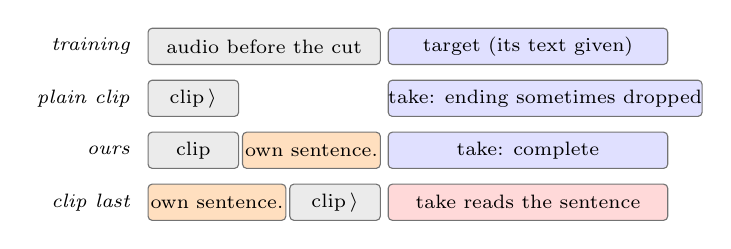
\begin{tikzpicture}[x=1cm,y=0.6cm,font=\scriptsize,
  b/.style={draw=black!55,rounded corners=1.5pt,minimum height=0.46cm,inner sep=0pt,align=center,anchor=west},
  lab/.style={anchor=east,font=\scriptsize\itshape}]
\node[lab] at (1.15,0) {training};
\node[b,fill=black!8,minimum width=2.95cm] at (1.25,0) {audio before the cut};
\node[b,fill=blue!12,minimum width=3.55cm] at (4.3,0) {target (its text given)};
\node[lab] at (1.15,-1.1) {plain clip};
\node[b,fill=black!8,minimum width=1.15cm] at (1.25,-1.1) {clip\,$\rangle$};
\node[b,fill=blue!12,minimum width=3.55cm] at (4.3,-1.1) {take: ending sometimes dropped};
\node[lab] at (1.15,-2.2) {ours};
\node[b,fill=black!8,minimum width=1.15cm] at (1.25,-2.2) {clip};
\node[b,fill=orange!25,minimum width=1.75cm] at (2.45,-2.2) {own sentence.};
\node[b,fill=blue!12,minimum width=3.55cm] at (4.3,-2.2) {take: complete};
\node[lab] at (1.15,-3.3) {clip last};
\node[b,fill=orange!25,minimum width=1.75cm] at (1.25,-3.3) {own sentence.};
\node[b,fill=black!8,minimum width=1.15cm] at (3.05,-3.3) {clip\,$\rangle$};
\node[b,fill=red!15,minimum width=3.55cm] at (4.3,-3.3) {take reads the sentence};
\end{tikzpicture}
\caption{Prompt layouts. In training the prompt is the audio preceding the target. A trimmed clip ends
mid-utterance ($\rangle$); prompt self-extension appends the model's own reading of a neutral sentence so
the prompt ends at a completed sentence. With the clip last, the model replays the extension.}
\label{fig:layout}
\end{figure}

\begin{algorithm}[t]
\caption{Prompt self-extension (once per voice)}\label{alg:ext}
\begin{algorithmic}[1]
\REQUIRE clip latents $c$ ($|c|\le 5$\,s), neutral sentence $s$, tries $K$
\FOR{$k=1..K$}
  \STATE $z_k \gets$ generate($s$ $\mid$ prompt $c$, seed $k$)
  \STATE $z_k \gets$ speech span of $z_k$ (+ one trailing frame)
\ENDFOR
\STATE $e \gets$ the $z_k$ of median speech length \COMMENT{no recogniser}
\STATE $p \gets [\,c \,;\, \text{last } (5\,\text{s} - |c|) \text{ of } e\,]$ \COMMENT{clip first, extension last}
\ENSURE prompt $p$, used for every later take of this voice
\end{algorithmic}
\end{algorithm}

The extension is kept as the model's own (normalised) latents, converted back to the codec space the
prompt is read in; decoding it to audio and re-encoding it worked less well in a Whisper-scored probe (\RES{0.286} vs
\RES{0.230} CER).
Choosing the take with a recogniser instead (lowest CER of the $K$) was not consistently
better (Table~\ref{tab:mech}); choosing it by speaker similarity is discussed below. The cost is $K$ short generations when a voice is added, and none per request: the extended prompt is
encoded once into the key--value cache that every unit already copies.

\textbf{Order.} With the clip placed \emph{after} the extension the prompt again ends abruptly, and the model
reads the extension sentence aloud instead of the text in \RES{94--99\%} of takes under both judges: the
take for the input \fa{«بله»} begins with \fa{«امروز هوا کمی سرد»}, the extension's opening words. The order
is therefore part of the method, not a detail.

\textbf{Controls.} Table~\ref{tab:mech} varies one thing at a time on the short development units
(180 paired takes per cell, consensus label). More real speech with the same abrupt ending (the clip twice)
does not help and hurts the male voice. The same extension cut after two thirds --- same voice, same kind of
latents, but ending mid-utterance --- multiplies failures by \RES{3--10}. Teacher-forcing a carrier word
before the text (continuation priming) has no effect, and conditioning each unit on the previous unit's last
2\,s (to carry prosody across joins) adds nothing over the extension and, alone, lowers UTMOS by
\RES{0.11}. Which sentence is read matters: of seven candidates,
two (A, chosen first and fixed before any held-out test, and G) help both voices, whether the take is chosen
with or without a recogniser; three hurt the male voice, among them a greeting (B) and two neutral statements
(E, F). Neither the end-of-speech timing nor the engine's acceptance rate of the probe takes predicted which
sentences work (rank correlations from \RES{$-$0.06} to \RES{$-$0.58}, inconsistent across voices), so the
sentence is a hyperparameter that needs a judge to choose; we report this as a limitation rather than tune
it on test data. Sentence G, the other one that helped on development data, carries over only partly to the
held-out set (male voice \RES{$-$1.5} points, CI \RES{[$-$3.3, +0.1]}; female voice unchanged).

\begin{table}[t]
\caption{Prompt variants on short dev units: consensus CER (failed takes of 180)}\label{tab:mech}
\centering
\setlength{\tabcolsep}{4pt}
\begin{tabular}{lcc}
\toprule
prompt & male, 1.36\,s clip & female, 2.0\,s clip \\
\midrule
clip (baseline) & \RES{.075 (18)} & \RES{.033 (7)} \\
clip twice & \RES{.136 (27)} & \RES{.034 (8)} \\
clip + ext.\ A & \RES{.045 (8)} & \RES{.011 (2)} \\
clip + ext.\ A, ASR-free take & \RES{.037 (4)} & \RES{.021 (5)} \\
clip + ext.\ A cut mid-sentence & \RES{.229 (48)} & \RES{.333 (72)} \\
ext.\ A + clip (clip last) & \RES{1.33 (169)} & \RES{1.38 (179)} \\
clip + carrier \fa{«خب»} primed & \RES{.072 (16)} & \RES{.027 (5)} \\
clip + ext.\ B (greeting) & \RES{.148 (30)} & \RES{.038 (7)} \\
clip + ext.\ C (short replies) & \RES{.077 (16)} & \RES{.032 (6)} \\
clip + ext.\ D (formal) & \RES{.117 (28)} & \RES{.036 (8)} \\
clip + ext.\ A + B & \RES{.098 (17)} & \RES{.026 (8)} \\
clip + ext.\ E (neutral, past) & \RES{.102 (23)} & \RES{.027 (6)} \\
clip + ext.\ F (neutral, one clause) & \RES{.099 (23)} & \RES{.034 (7)} \\
clip + ext.\ G (neutral, habitual) & \RES{.043 (8)} & \RES{.019 (4)} \\
\bottomrule
\end{tabular}
\end{table}

\textbf{Held-out results.} Two test sets were never used for any choice above. \emph{Short:} 60 new
sentences of 1--5 words (50 Persian, 5 English, 5 mixed), rendered through the full production path (front
end, chunking, three-attempt signal retry, stitching). \emph{Bench:} 79 mixed cases (prose, numbers, dates,
English, code-mixed, acronyms, punctuation, 12 paragraphs). Table~\ref{tab:held} pairs renders by case and
seed. On short sentences, pooled over the three voices, failed renders halve (\RES{24 $\to$ 12} of
\RES{900} Persian renders; consensus error \RES{3.2\% $\to$ 2.2\%}, CI \RES{[$-$1.7, $-$0.4]} points). The
gain is significant for the 1.36\,s clip that the engine ships as its default (\RES{6.0\% $\to$ 3.9\%}) and
small for the two voices that were already near the floor. UTMOS \cite{utmos2022} rises for every voice
(\RES{+0.09 to +0.17}). Speaker similarity to the clip (WeSpeaker \cite{wespeaker2023}) is unchanged for both
male voices but drops by \RES{0.03} for the female voice, whose reading of the extension drifts from the
clip; this is the method's cost. On the bench, where most units are long, the final configuration also lowers the
Persian consensus error (\RES{2.9\% $\to$ 2.3\%}, CI \RES{[$-$1.0, $-$0.1]} points), including numbers and
dates; with Whisper alone over all 237 renders the change is not significant (\RES{5.65\% $\to$ 5.05\%}),
failed renders stay at \RES{4}, and English cases are unchanged because they keep the plain clip (applying
the Persian extension to English sentences had made acronym cases drift, \RES{6.1\% $\to$ 12.1\%}, n.s.).
Speaker similarity drops slightly (\RES{$-$0.011}). An unplanned effect is at chunk joins: the pitch reset
between consecutive units of one sentence falls from \RES{5.2} to \RES{3.9} semitones and the
utterance-final fall inside sentences from \RES{1.9} to \RES{1.3}, i.e.\ units sound less like separate
sentences.

\textbf{New, tightly cut clips.} The voices above were chosen before this work. As a final check we took
three real 2.6\,s recordings from GPTInformal (CC0) that the corpus cut 0.02\,s after the last sound --- one
at the end of a sentence, one at a comma, one in the middle of a clause --- and used them as voice prompts
for the short set, building their extensions with Algorithm~\ref{alg:ext} and no further tuning. The
mid-clause clip is nearly unusable on its own (consensus error \RES{44\%}, \RES{70} of \RES{150} renders
failed) and becomes ordinary with the extension (\RES{3.0\%}, \RES{4} failed); the comma clip halves its
error and the sentence-final clip improves slightly (Table~\ref{tab:held}). Pooled, failures fall from
\RES{96} to \RES{19} of \RES{450}. This is the prediction of the mechanism: the less finished the prompt's
ending, the larger the gain.

\textbf{Which take of the extension.} The extension take matters as well as the sentence: two
median-length choices of sentence A gave \RES{4} and \RES{13} failures on the male development units. Keeping
instead the take whose WeSpeaker embedding is closest to the clip (still no recogniser) removes the speaker
cost --- pooled similarity \RES{+0.009} instead of \RES{$-$0.012}, the female voice \RES{+0.010} instead of
\RES{$-$0.030} --- and gives the largest UTMOS gain (\RES{+0.18}), but a smaller error reduction
(\RES{$-$0.7} points, CI \RES{[$-$1.6, +0.1]}). The choice of take is therefore a knob between intelligibility
and voice fidelity; Table~\ref{tab:held} reports both.

\textbf{Retries become unnecessary.} On short sentences the engine's three-take rule spends \RES{2.1}
generations per unit (its duration window rejects many good short takes), yet with the plain clip one take
instead of three changes nothing measurable (\RES{6.0\% $\to$ 5.9\%}). With the extension and a single take
the error is \RES{4.1\%} --- \RES{$-$1.9} points against today's three-take default (CI \RES{[$-$3.3,
$-$0.6]}) --- UTMOS is higher (\RES{+0.08}), and the engine does \RES{1.0} instead of \RES{2.1} generations per
unit (\RES{1.06\,s} instead of \RES{1.88\,s} of CPU per short sentence in our runs). On a third test set,
40 assistant-style replies written for this check (1--15 words, five with English terms), the recommended
configuration (extension for Persian sentences, one take) is not worse on any measure --- consensus error
\RES{3.2\% $\to$ 2.6\%}, Whisper failures \RES{12 $\to$ 7} of 120, UTMOS and speaker similarity unchanged ---
while doing \RES{28\%} fewer generations (\RES{1.38 $\to$ 1.00} per unit).

\begin{table}[t]
\caption{Held-out results with the final configuration (ASR-free extension), paired renders; change with
95\% case-bootstrap CI}\label{tab:held}
\centering
\setlength{\tabcolsep}{2.5pt}
\begin{tabular}{lccc}
\toprule
metric & clip & clip+ext & change [CI] \\
\midrule
\multicolumn{4}{l}{\emph{short set, 60 sentences $\times$ 6 seeds, male 1.36\,s clip}} \\
CER, consensus (fa, 300) & \RES{.060} & \RES{.039} & \RES{$-$.021 [$-$.036, $-$.008]} \\
failed renders (fa, 300) & \RES{19} & \RES{8} & \\
CER, Whisper only (fa) & \RES{.316} & \RES{.250} & \RES{$-$.066 [$-$.107, $-$.024]} \\
UTMOS (360) & \RES{3.01} & \RES{3.12} & \RES{+.12 [+.04, +.20]} \\
speaker sim.\ (360) & \RES{.195} & \RES{.193} & \RES{$-$.001 [$-$.016, +.013]} \\
\multicolumn{4}{l}{\emph{same, female 2.0\,s clip}} \\
CER, consensus (fa, 300) & \RES{.020} & \RES{.016} & \RES{$-$.004 [$-$.009, +.002]} \\
UTMOS (360) & \RES{3.42} & \RES{3.59} & \RES{+.17 [+.10, +.24]} \\
speaker sim.\ (360) & \RES{.215} & \RES{.185} & \RES{$-$.030 [$-$.046, $-$.015]} \\
\multicolumn{4}{l}{\emph{same, male 5.1\,s clip}} \\
CER, consensus (fa, 300) & \RES{.017} & \RES{.010} & \RES{$-$.007 [$-$.017, +.004]} \\
UTMOS (360) & \RES{3.29} & \RES{3.38} & \RES{+.09 [+.04, +.15]} \\
speaker sim.\ (360) & \RES{.276} & \RES{.270} & \RES{$-$.006 [$-$.021, +.010]} \\
\multicolumn{4}{l}{\emph{all three voices pooled (fa, 900; UTMOS and speaker sim.\ over 1080)}} \\
CER, consensus & \RES{.032} & \RES{.022} & \RES{$-$.011 [$-$.017, $-$.004]} \\
failed renders & \RES{24} & \RES{12} & \\
UTMOS / speaker sim.\ change & & & \RES{+.13 / $-$.012} \\
\multicolumn{4}{l}{\emph{pooled, speaker-matched extension take}} \\
CER, consensus & \RES{.032} & \RES{.025} & \RES{$-$.007 [$-$.016, +.001]} \\
failed renders & \RES{24} & \RES{20} & \\
UTMOS / speaker sim.\ change & & & \RES{+.18 / +.009} \\
\midrule
\multicolumn{4}{l}{\emph{short set, 3 seeds, three new real 2.6\,s clips cut 0.02\,s after speech}} \\
CER, consensus, clip ends a sentence & \RES{.036} & \RES{.020} & \RES{$-$.017 [$-$.044, +.008]} \\
CER, consensus, clip ends at a comma & \RES{.161} & \RES{.088} & \RES{$-$.073 [$-$.185, +.020]} \\
CER, consensus, clip ends mid-clause & \RES{.441} & \RES{.030} & \RES{$-$.411 [$-$.546, $-$.288]} \\
pooled failed renders (fa, 450) & \RES{96} & \RES{19} & \RES{$-$.167 [$-$.233, $-$.106]} \\
UTMOS change (3 clips) & & & \RES{+.34, +.32, +.69} \\
speaker sim.\ change (3 clips) & & & \RES{+.028, +.002, $-$.042} \\
\midrule
\multicolumn{4}{l}{\emph{bench, 79 cases $\times$ 3 seeds, male 1.36\,s clip, final configuration}} \\
CER, consensus (fa, 165) & \RES{.029} & \RES{.023} & \RES{$-$.006 [$-$.010, $-$.001]} \\
CER, Whisper (all 237) & \RES{.057} & \RES{.051} & \RES{$-$.006 [$-$.015, +.001]} \\
failed renders (237) & \RES{4} & \RES{4} & \\
UTMOS (237) & \RES{3.28} & \RES{3.28} & \RES{$-$.01 [$-$.04, +.02]} \\
speaker sim.\ (237) & \RES{.286} & \RES{.276} & \RES{$-$.011 [$-$.017, $-$.004]} \\
pitch reset at joins (st) & \RES{5.25} & \RES{3.92} & \RES{$-$1.33 [$-$1.95, $-$0.77]} \\
mid-sentence final fall (st) & \RES{1.93} & \RES{1.28} & \RES{$-$0.65 [$-$1.22, $-$0.05]} \\
\bottomrule
\end{tabular}
\end{table}

\section{Discussion and limitations}
\textbf{Why the ending matters.} The training cut makes the prompt the audio \emph{before} the target, so
the model learns to continue from wherever the prompt stops. A prompt that stops on a completed sentence
asks for a new one; a prompt that stops mid-phrase --- a tightly trimmed clip, a clip after an extension, an
extension cut short --- asks the model to finish something it was not given the words for, and the result
is a replay of the prompt or a short target with its ending dropped. Self-extension is one way to make every
voice end the same, well-formed way without asking users for longer or pause-padded recordings; padding the
clip with silence alone was inconsistent across voices in our probes.

\textbf{Limitations.} One model and six voice clips (three from one speaker); results may differ for discrete-token or
attention-aligned TTS. Intelligibility is measured with recognisers, which is why we report two and their
floor on real speech. A first blind A/B test (one listener, one male voice, 60 pairs) heard no difference
in preference (\RES{same 33, base 15, extension 12; sign test $p=.70$}) and marked word errors in \RES{7 base
and 5 extended} renders (\RES{3 vs.\ 1} on Persian-only sentences), but its error marks and the
recognisers' failures fell on different takes (\RES{0 of 21 in common}); the intelligibility gains above
are therefore recogniser-measured and await a larger listening test. The
extension sentence is a hyperparameter: of seven candidates two helped both voices, no simple property
predicted which, and we fixed it on development data. English sentences, read through mapped Persian phonemes, did not benefit from a Persian
extension (acronym cases drifted, \RES{6.1\% $\to$ 12.1\%}, n.s.); keeping the plain clip for sentences the
front end marks as English removes this (\RES{6.1\%}, identical renders), so the engine extends the prompt
for Persian and code-mixed sentences only. The extension changes the prosody of every unit, not only short
ones; we measured joins and UTMOS but not long-form drift.

\section{Conclusion}
Short inputs are where a small CPU TTS model fails, and a single ASR judge overstates how often. Signals
available without a recogniser locate risky units but not failed takes, so retries without a recogniser
mostly add cost. Making the voice prompt end the way training prompts end --- with the model's own reading of
one neutral sentence after the clip --- halves failed short renders on held-out data, rescues clips that
are cut mid-utterance, raises UTMOS, smooths chunk joins and costs nothing per request; it lets the engine drop its retries, halving the generation work
while making fewer errors. Its price, a small loss of speaker similarity for one of three voices, disappears when the
extension take is chosen by speaker similarity, at part of the intelligibility gain. Code,
sentence sets and labels will be released with the paper \RES{[URL]}.

\bibliographystyle{IEEEtran}
\bibliography{refs}
\end{document}
